\section{Diskrete Fouriertransformation mit ANN\label{ml:dft-with-ann}}
\rhead{DFT mit ANN}

Die \emph{diskrete Fouriertransformation} (DFT) einer Zahlenreihe $x_n \in \{ x_0, x_1, \cdots, x_{N-1}\}$
mit $N$ Elementen kann mit
\begin{equation}
    c_k = \frac{1}{N} \sum_{n=0}^{N-1} x_n e^{\normalsize -jk\frac{2\pi}{N}n}
\end{equation}
berechnet werden, oder in vektorschreibweise
    \begin{equation}
    c_k = \begin{pmatrix}
        x_0\\
        x_1\\
        \vdots\\
        x_{N-1}
    \end{pmatrix} \cdot
    \frac{1}{N} \begin{pmatrix}
        e^{-j \omega_k 0} \\
        e^{-j \omega_k 1} \\
        \vdots \\
        e^{-j \omega_k (N-1)} \\
    \end{pmatrix}
    \qquad \text{mit}\qquad \omega_k = \frac{2\pi k}{N}.
    \label{ml:dft-with-ann:dft:vector}
\end{equation}

Die einzelnen $x_n$ werden mit einem komplexen Koeffizienten gewichtet und anschliessend
summiert. In der Vektorschreibweise wird dieser Effekt mit dem Skalarprodukt erzielt. Man
erkennt, dass dies ein linearer Zusammenhang ist.

Um uns auf die reellen Zahlen zu bschränken, wird \eqref{ml:dft-with-ann:dft:vector} in
die Kosinus-Anteile $a_k = 2{\rm Re}(c_k)$ und Sinus-Anteile $b_k = -2{\rm Im}(c_k)$
unterteilt:
\begin{equation}
    a_k = \vec x \cdot \frac{2}{N} \begin{pmatrix}
        1\\
        \cos(\omega_k 1)\\
        \vdots\\
        \cos(\omega_k (N-1))
    \end{pmatrix}
    = \vec x \cdot \vec \theta_{k,a}
    \quad \text{und} \quad
    b_k = \vec x \cdot \frac{-2}{N} \begin{pmatrix}
        0\\
        \sin(\omega_k 1)\\            
        \vdots\\
        \sin(\omega_k (N-1))
    \end{pmatrix}
    = \vec x \cdot \vec \theta_{k,b}.
\end{equation}
Beide Teile sind bis auf die Koeffizienten genau gleich. Sie können  in der Form des mehrdimensionalen linearen
Modells \eqref{ml:ann:linear-unit} als
\begin{equation}
    \vec a = \begin{pmatrix}a_0\\ \vdots \\ a_{N-1} \end{pmatrix} = \begin{pmatrix}
        \vec \theta_{0,a} & \vec \theta_{1,a} & \cdots & \vec \theta_{N-1,a}
    \end{pmatrix} \vec x
    = {\bm \thetaup}_{a} \vec x
    \quad\text{und}\quad
    \vec b = {\bm \thetaup}_{b} \vec x
\end{equation}
geschrieben werden. Die konstanten Anteile entfallen.

In Abb. \ref{fig:ml:dft-with-ann:linear} ist das Netz für die Kosinus-Anteile abgebildet.
Als Übertragungsfunktion wurde für die Linearität die Identitätsfunktion $f(x) = x$ gewählt. Das Netz ist
also linear und nicht einmal affin (alle Bias-Werte sind Null). Ein analoges Netz kann
auch für die Sinus-Anteile erstellt werden. Alternativ können die Sinus-Koeffizienten aus
den Kosinus-Koeffizienten mit dem Zusammenhang
\begin{equation}
    \frac{N}{2} \arccos(\theta_{kn,a}) = \frac{N}{-2} \arcsin(\theta_{kn,b}) \quad \iff \quad
    \theta_{kn,b} = -\sin(\arccos(\theta_{kn,a}))
\end{equation}
berechnet werden.

\begin{figure}
    \centering
    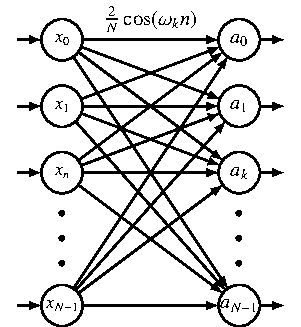
\includegraphics[scale=0.8]{papers/ml/images/ann_dft_linear.pdf}
    \caption{Lineares Netzwerk für die DFT.}
    \label{fig:ml:dft-with-ann:linear}
\end{figure}

Man kann erkennen, das so ein Netz unseren Fall der linearen Regression
(\ref{ml:regression}) exakt wiederspiegelt. Die Koeffizienten $\vec \theta_{k,a}$ und
$\vec \theta_{k,b}$ können also mit herkömmlichem Gradient-Descent gelernt werden, und das
sogar in endlich vielen Schritten, exakt.

Leider haben wir mit dieser Methodik überhaupt nichts gewonnen. Die Koeffizienten müssen
zwar nur \emph{einmal} gelernt werden bei gleichbleibendem $N$, um aber die
fouriertransformierten Werte $c_k$ zu berechnen, müssen immer noch zwei volle
Matrix-Vektor multiplikationen durchgeführt werden. Hier ist die schnelle
Fouriertransformation bei weitem überlegen.

Die Frage, ob es möglich ist mit einem künstlichen neuronalen Netzwerk die Fouriertransformation zu
berechnen können wir totzdem bejahen. Denn so ein lineares Netzwerk \emph{ist} ein FFANN,
auch wenn ein Spezialfall.

Möchte man, dass ein Modell die Fouriertransformation selber lernt, wenn es
sie benötigt, ist das mit einem nichtlinearen FFANN schlecht realisierbar und sehr
aufwändig. Ein besserer Ansatz bietet \cite{ml:pmlr-v97-dao19a}, wobei durch ein geschickt
aufgebautes lineares Netzwerk mit schwachbesetzten Schichten, Faktorisierungen von einer
vielzahl der linearen Transformationen gelernt werden können. \cite{ml:pmlr-v97-dao19a}
zeigt also, dass ein ANN mit geschicktem Aufbau in der Lage ist ein fast beliebigen
schnellen linearen Transformations-Algorithmus (zum Beispiel die FFT) aus Daten zu rekonstruieren.